\documentclass[11pt,a4paper]{article}
\usepackage[utf8]{inputenc}
\usepackage[margin=2.2cm, top=2.8cm, bottom=2.8cm]{geometry}
\usepackage{fancyhdr}
\usepackage{tabularx}
\usepackage{booktabs}
\usepackage{listings}
\usepackage{xcolor}
\usepackage{graphicx}
\usepackage[hidelinks]{hyperref}
\usepackage{titlesec}
\usepackage{colortbl}

% --- THGA Lecture Color Theme ---
\definecolor{thgablue}{HTML}{003366}
\definecolor{thgared}{HTML}{A00000}
\definecolor{codebg}{HTML}{F6F8FA}
\definecolor{tableheader}{HTML}{E8EEF5}
\definecolor{boxframe}{HTML}{B8D0E8}
\definecolor{boxbg}{HTML}{F0F5FA}

% --- Section Styling ---
\titleformat{\section}
  {\color{thgablue}\normalfont\Large\bfseries}
  {\color{thgablue}\thesection}{1em}{}[\color{thgablue}\titlerule]

\titleformat{\subsection}
  {\color{thgablue}\normalfont\large\bfseries}
  {\color{thgablue}\thesubsection}{1em}{}

% --- Header / Footer ---
\pagestyle{fancy}
\fancyhf{}
\lhead{\small\textbf{\color{thgablue}CounterStock} --- Operations Manual}
\rhead{\small\color{gray}Baha Eddine Nabhan \quad September 2026}
\lfoot{\small\texttt{\color{thgared}baha@counterstock.local}}
\cfoot{\small\color{gray}THGA Bochum}
\rfoot{\small\textbf{\color{thgablue}\thepage}}
\renewcommand{\headrulewidth}{0.6pt}
\renewcommand{\footrulewidth}{0.4pt}

% --- Listing Style ---
\lstset{
    basicstyle=\ttfamily\footnotesize,
    backgroundcolor=\color{codebg},
    frame=leftline,
    framerule=2pt,
    rulecolor=\color{thgablue},
    breaklines=true,
    numbers=left,
    numberstyle=\tiny\color{gray},
    keywordstyle=\color{thgared}\bfseries,
    commentstyle=\color{gray}\itshape,
    stringstyle=\color{thgablue}
}

\begin{document}

% --- Title Block ---
\noindent
{\LARGE\textbf{\color{thgablue}CounterStock: User Manual}} \hfill {\large\textbf{\color{thgared}Winter Semester 2026}}\\[0.2cm]
{\small POS Operations, Inventory Control \& Dispatch} \hfill {\small THGA Bochum}\\
{\small Instructor: Stephan B\"okelmann} \hfill {\small Informationstechnik und Digitalisierung}\\[0.25cm]
{\color{thgablue}\hrule height 1.5pt}

% --- Centered Table of Contents Block ---
\vspace*{\fill}

\begin{center}
\parbox{0.92\textwidth}{
  \renewcommand{\contentsname}{\centering\LARGE\color{thgablue}Table of Contents}
  \tableofcontents
}
\end{center}

\vspace{1.2cm}
\noindent\fcolorbox{boxframe}{boxbg}{%
\parbox{0.97\textwidth}{%
\textbf{\color{thgablue}Notice for Terminal Operators:} Keep this document accessible at the cashier terminal. It covers daily setup, live portion tracking, transaction conflict diagnosis, and delivery intake workflows.
}}

\vspace*{\fill}

\newpage

\section{Motivation and Operational Context}
In standard snack bars and fast-service gastronomy, point-of-sale terminals operating independently from physical storage produce phantom orders: cashiers accept payments for items whose ingredients are depleted. This results in order cancelations, refund overhead, and lost customer confidence.

\textbf{\color{thgared}CounterStock} resolves this problem at the database boundary. The desktop client queries dynamically computed portions based on physical ingredient stocks, forbidding cashiers from placing orders when even a single recipe component is exhausted.

\vspace{0.3cm}
\noindent\fcolorbox{boxframe}{boxbg}{%
\parbox{0.97\textwidth}{%
\textbf{\color{thgablue}Core Principle:} Cashiers do not input abstract numbers; they operate directly against a live view of real kitchen warehouse availability.
}}
\vspace{0.3cm}

\section{System Requirements and Installation}
\subsection{Hardware and Network Prerequisites}
\begin{itemize}
    \item \textbf{Operating System:} Ubuntu Linux 22.04 LTS / 24.04 LTS (x86\_64)
    \item \textbf{Display:} Minimum resolution of 1024$\times$768
    \item \textbf{Network:} HTTP connectivity to the CounterStock API host (\texttt{http://localhost:8000})
\end{itemize}

\subsection{Native Debian Package Deployment}
The desktop GUI is distributed as an independent, pre-compiled Debian package containing the necessary Python runtime and Tkinter bindings:
\begin{lstlisting}[language=bash]
# Install native .deb archive
sudo dpkg -i db-frontend_0.1.0_amd64.deb

# Launch application via system path
db-frontend
\end{lstlisting}

\section{Application Setup \& Connection}
Upon launching \texttt{db-frontend}, a modal handshake dialog prompts the cashier or manager to provide server coordinates.

\begin{figure}[h!]
\centering
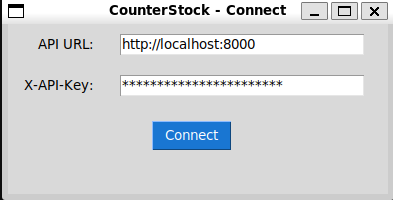
\includegraphics[width=0.6\textwidth]{screenshot_connect.png}
\caption{\color{thgablue}Modal Handshake: Server Base URL and API Token Entry}
\end{figure}

\begin{enumerate}
    \item \textbf{API URL:} Address of the backend service (default: \texttt{http://localhost:8000}).
    \item \textbf{X-API-Token:} The security token issued to the terminal (\texttt{secret\_counterstock\_key}).
    \item Click \textbf{\color{thgablue}Connect}. When verified, the terminal transitions to active status.
\end{enumerate}

\noindent\textbf{\color{thgared}Diagnostic Note:} If the dialog reports a connection error, verify that the Docker Compose backend cluster is running (\texttt{docker compose ps}) and port 8000 is open.

\section{Cashier Operations: Menu \& Live Ordering}
\subsection{Real-Time Portion Calculation}
Navigate to the \textbf{Menu \& Ordering} tab. The table displays active menu offerings.

\begin{figure}[h!]
\centering
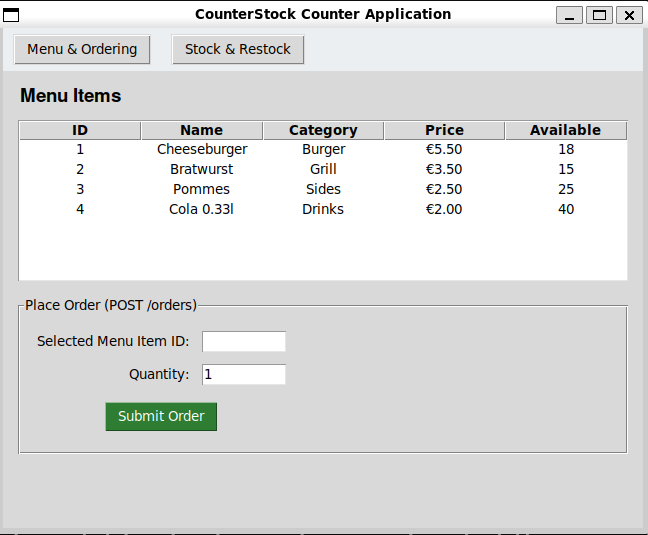
\includegraphics[width=0.72\textwidth]{screenshot_menu.png}
\caption{\color{thgablue}Live POS Catalog Showing Dynamically Computed Available Portions}
\end{figure}

The \textbf{Available} column is not manually set. It is computed in real-time from the bottleneck ingredient:
\begin{equation}
\text{Available Portions} = \min_{r \in \text{Ingredients}} \left( \left\lfloor \frac{\text{Stock Quantity}_r}{\text{Required Quantity}_r} \right\rfloor \right)
\end{equation}

\subsection{Submitting Customer Orders}
\begin{enumerate}
    \item Enter the \textbf{Menu Item ID} (e.g., \texttt{1} for Cheeseburger).
    \item Enter the requested \textbf{Quantity}.
    \item Click \textbf{\color{thgablue}Submit Order}.
    \item \textbf{Success:} A green confirmation popup indicates the Order ID and calculated subtotal. The available portion count drops immediately across terminals.
\end{enumerate}

\subsection{Handling Out-of-Stock Rejections}
If a transaction requests more items than ingredients permit, the server rejects the order:

\begin{figure}[h!]
\centering
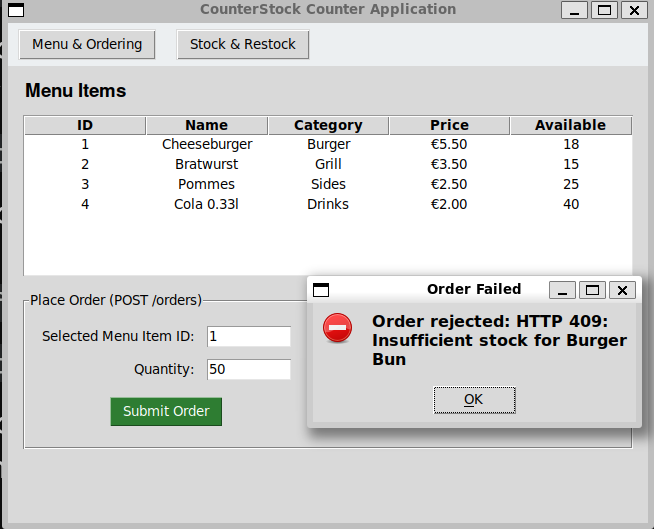
\includegraphics[width=0.62\textwidth]{screenshot_error.png}
\caption{\color{thgared}Out-of-Stock Conflict Rejection Notice (HTTP 409)}
\end{figure}

The cashier receives an explicit error dialog: \texttt{\color{thgared}HTTP 409 Conflict: Insufficient stock for [Ingredient]}. Offer alternative dishes or request an ingredient restock.

\newpage
\section{Stock Monitoring and Delivery Intake}
Switch to the \textbf{Low Stock} tab. Ingredients at or below their configured safety margin appear automatically.

\begin{figure}[h!]
\centering
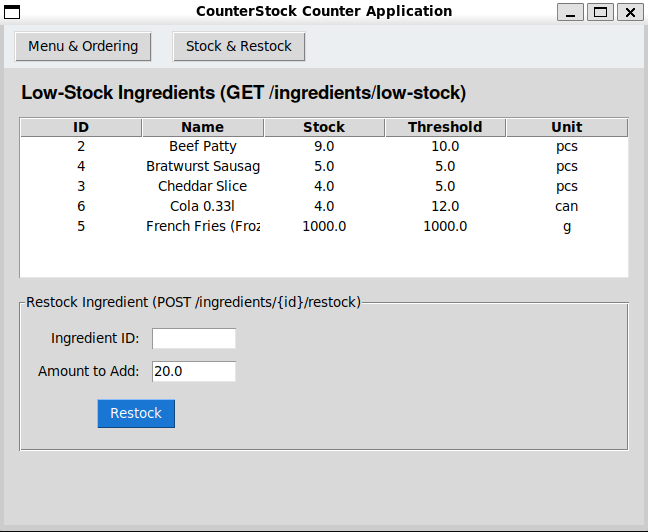
\includegraphics[width=0.72\textwidth]{screenshot_restock.png}
\caption{\color{thgablue}Low-Stock Threshold Alert Dashboard}
\end{figure}

\subsection{Recording Incoming Deliveries}
\begin{enumerate}
    \item Select the ingredient from the Low Stock grid.
    \item Enter the received delivery amount in the text field.
    \item Click \textbf{\color{thgablue}Restock Inventory}. The menu catalog instantly reflects the increased available portions.
\end{enumerate}

\clearpage

\section{Frequently Asked Questions (FAQ)}
\begin{description}
    \item[\color{thgablue}Q: Why does the login screen report "Connection Refused"?]~\\
    The backend API is not listening. Run \texttt{docker compose up -d} inside \texttt{counterstock-backend} and confirm health via \texttt{curl http://localhost:8000/menu}.
    \item[\color{thgablue}Q: Can inventory balances drop below zero?]~\\
    No. The database enforces this via a \texttt{CHECK (stock\_quantity >= 0)} constraint. Overselling is blocked by the transactional engine.
    \item[\color{thgablue}Q: What happens if the cashier window closes unexpectedly?]~\\
    All confirmed sales are committed to PostgreSQL. No local state is lost; reopening \texttt{db-frontend} restores the latest live values.
\end{description}

\end{document}
